\documentclass[a4paper,ngerman,landscape]{scrartcl}

\usepackage[utf8]{inputenc}

\usepackage[ngerman]{babel}
\usepackage{hyperref}

\usepackage{graphicx}

\usepackage[protrusion=true,expansion=true]{microtype}

\usepackage{lmodern}
\usepackage{tabto}

\setlength\parskip{\medskipamount}
\setlength\parindent{0pt}

\usepackage{geometry}
\geometry{tmargin=0.5cm,bmargin=1.0cm,lmargin=2.5cm,rmargin=2.5cm}

\pagestyle{empty}

\begin{document}

\begin{center}
  \huge
  Mittwoch, 2. Oktober 2013, 10:00 Uhr, 2004/L1 \\
  \mbox{\textbf{Johannes Sedlmeir: Konstruktive Mathematik und Quantenmechanik II}}
  \vfill
  
\includegraphics[scale=1.2]{schroedingers-katze}
  \vfill

  \Large
  \begin{minipage}{0.94\textwidth}
    \setlength\parskip{\medskipamount}
    Ein quantenmechanisches System kann durch eine nichtkommutative
    $C^\star$-Algebra beschrieben werden, \mbox{deren} selbstadjungierte Elemente den
    Observablen des Systems entsprechen. Anders als in der klassischen Mechanik
    können den Observablen aber keine konsistenten Messwerte zugeordnet werden;
    in der Quantenmechanik ist das nur für Observablen aus \emph{kommutativen}
    Unteralgebren möglich.

    Dieser Vortrag setzt den Vortrag von vor zwei Wochen fort. Wenn noch Zeit
    ist, werden wir auch den \emph{Bohr-Topos} einführen, eine Art
    nichtkommutativen Raum, aus dessen interner Sicht die $C^\star$-Algebra
    eines quantenmechanischen Systems kommutativ erscheint und das System daher
    in einem gewissen Sinn wie ein klassisches System behandelt werden kann.
  \end{minipage}
\end{center}

\newpage

\begin{center}
  \huge
  Mittwoch, 2. Oktober 2013, 12:15 Uhr, 2004/L1 \\
  \textbf{Kathrin Gimmi: Knotentheorie III}
  \vfill
  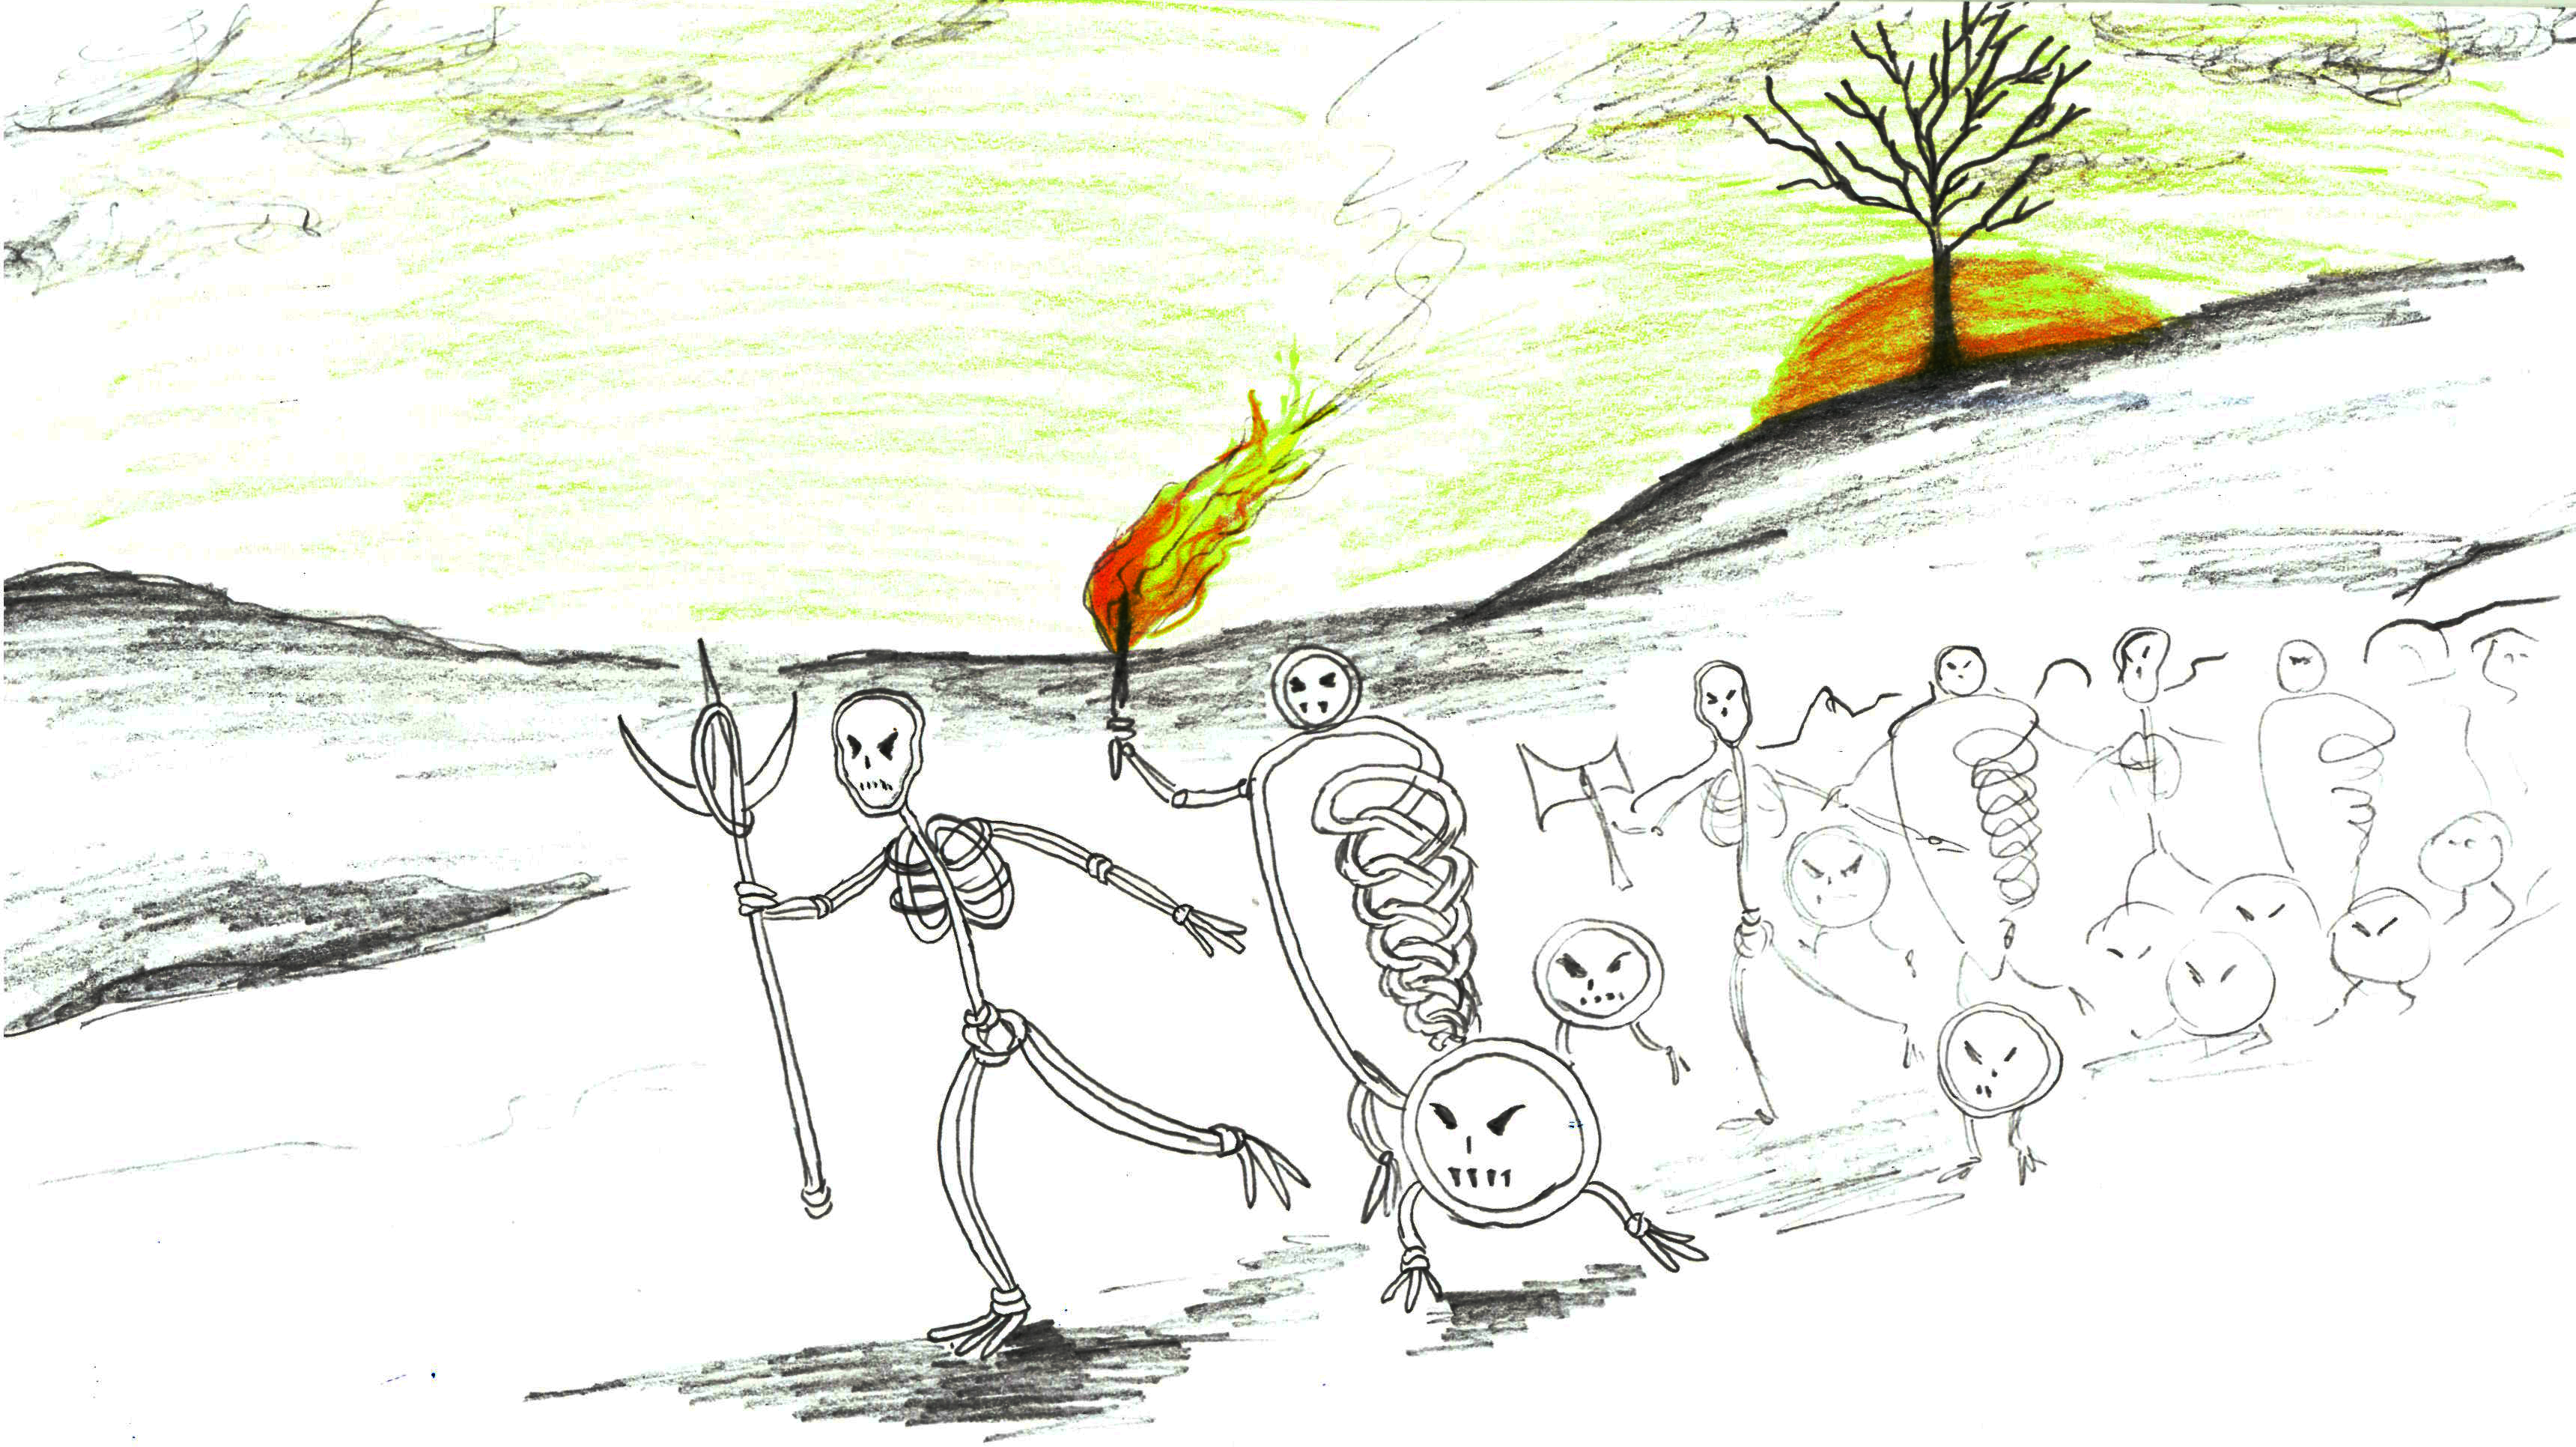
\includegraphics[scale=0.6]{knotenarmee-duester-farbkorrigiert}
  \vfill

  \Large
  \begin{minipage}{0.94\textwidth}
    \setlength\parskip{\medskipamount}
    Eine grundlegende Möglichkeit, um einen vorgegebenen Knoten zu verstehen,
    besteht darin, das Komplement des Knotens im umgebenden dreidimensionalen
    Raum zu studieren. Dieses hat nämlich eine nichttriviale
    Struktur: Viele Schleifen lassen sich nicht auf einen Punkt zusammenziehen,
    und es gibt algebraische Relationen zwischen verschiedenen Schleifen. Diese
    Informationen werden übersichtlich in der \emph{Knotengruppe} kodiert.

    Im Vortrag werden wir dieses Phänomen verstehen und
    den \emph{Wirtinger-Algorithmus} kennenlernen, mit dessen Hilfe man aus einer
    zweidimensionalen Projektion des Knotens sehr einfach seine Knotengruppe
    bestimmen kann.
  \end{minipage}
\end{center}

\hfill\small Skript und Übungsblätter: \url{http://pizzaseminar.speicherleck.de/}
\end{document}
